% !TeX root = ../mythesis.tex
% !TeX encoding = UTF-8
% !TeX spellcheck = en_US

\chapter{Data Structures and Algorithms}



% \section{Data structures}

% \begin{enumerate}
% 	\item Trees as first order literals, i.e.\ the root symbol is either a (negated) predicate symbol or the (negated) equality symbol.
% 	\item Multisets of literals for first order clauses
% 	\item Sets for Problems, i.e.~sets of clauses
% \end{enumerate}

% \subsection{Terms, Atoms, and Literals}

% The recursive definition of the syntax of terms, atoms and literal suggests a tree data structure.


% \begin{tikzpicture}[->,>=stealth',level/.style={sibling distance = 2cm/#1,
% 	level distance = 0.8cm}]

% \node { \( \lnot \) }
% 	child {
% 		node { \( \mP \) }
% 		child { node {\( x \)} }
% 		child { node {\( \mf \)}
% 			child { node {\( x \)} }
% 		}
% 	}
% ;
% \end{tikzpicture}

% \begin{tikzpicture}
% \draw (0,0) rectangle (1,1);
% \draw (0.1,0.1) rectangle (1cm,1cm);

% \draw (0,0) to (1,1);
% \end{tikzpicture}

% \subsection{Sets}

% Clauses are defined as multisets of literals.


\section{Saturation Basics}\label{sec:saturation:basics}

In the examples of Chapter~\ref{chapter:automation},
we just applied derivation rules
to haphazardly chosen pairs of clauses
to infer new clauses
until we could conclude unsatisfiability.
%
In practice, such an approach may fail for an unsatisfiable set of clauses
simply because an important clause pairing is overlooked
and an infinite number of inferences can be drawn
from a satisfiable subset of clauses.
%
In Chapter~\ref{chapter:completeness}, on the other hand,
we relied on a fair ---
i.e.\ every non-redundant clause will be processed eventually ---
saturation process to show completeness of \InstGenEQ{}.

For now we will ignore possible simplifications of the set of clauses.
In Section~\ref{sec:given:clause:algorithm}
we will combine the given clause algorithm
and a basic selection strategy to a a simple and fair saturation process
that eventually determines all possible derivate clauses
with respect to ordered resolution.
Surprisingly the same approach will fail easily for \InstGen{}.
We consider a better suited bookkeeping of processed clauses and literals
in Section~\ref{sec:selected:literals:bookkeeping}.


% Both algorithms are just only building blocks for fair saturation strategies as we outline in Section~\ref{sec:fair:saturation:strategies:basics}

\subsection{Given Clause Algorithm}\label{sec:given:clause:algorithm}

The given clause algorithm is originated in the set of support strategy~\cite{Wos:1965:ECS:321296.321302}. (todo: Otter and discount loops~\cite{DBLP:conf/cade/SchulzM16})
%\cite{10.1007/978-3-319-40229-1_23, DBLP:conf/cade/SchulzM16})

\begin{procedure}[Given Clause Algorithm]\label{proc:given:clause:algorithm}
	We start with an empty set \( P \) of \coloremph{processed} clauses \( P \)
	and the original set of \coloremph{unprocessed} clauses \( U = S \),
	e.g.\ a set of axioms and a negated conjecture.
	\begin{enumerate}
		\item[\jek] Whenever we can conclude unsatisfiability of the original set of clauses \( S \),
		we exit the procedure with \( \lnot\SAT \).
		\setcounter{enumi}{0}
		\item If there are no unprocessed clauses,
		we exit and return \SAT{}.
		\item We select the \coloremph{best} unprocessed clause --- the now given clause \( G  \) --- and remove it from the unprocessed clauses. \hfill\jek{}
		\item We iterate over the processed clauses and check for applicable inference rules
		for each pair \( (C, G) \subseteq P \times \{ G \} \) of a processed and the given clause
		to derive additional clauses which we add to the set of unprocessed clauses. \hfill\jek{}
		\item We add the given clause to the set of processed clauses.
		We continue with step 1.
	\end{enumerate}
\end{procedure}

(In the following examples the given clause is boxed,
the processed clauses are left of the given clause,
and the unprocessed clauses are right of the given clause.
Each line represents one iteration of the procedure.)

A crucial part is the selection of the “best” unprocessed clause.
At least we have to ensure that any (non-redundant) clause is selected eventually.
Otherwise we may stay in a satisfiable subset of the set of clauses
as we demonstrate in the following silly example with respect to resolution.
\begin{example}[Insufficient clause selection]
	We process the clearly unsatisfiable set of clauses
	\( S = \{
		\msucc(x)\mNE \msucc(y)\lor {x\mEQ y},
		\msucc(x_2)\mNE x_2, \msucc(x')\mEQ x'
		\} \)
	and always select the \coloremph{newest} unprocessed clause as the “best” clause
	after we have moved the first clause to the processed clauses.

	\begin{align*}
		(k=1)\quad
		&\boxed{\msucc(x)\mNE \msucc(y)\lor {x\mEQ y}} &
		&&
		&{ \msucc^1(x_2)\mNE \msucc^0(x_2) },\ { \msucc(x')\mEQ x' }
		\\
		(k=2)\quad
		&\msucc(x)\mNE \msucc(y)\lor \underline{x\mEQ y} &
		&&
		&\boxed{ \msucc^1(x_2)\mNE \msucc^0(x_2) }\ \ldots
		\\
		(k=3)\quad
		&\msucc(x)\mNE \msucc(y)\lor \underline{x\mEQ y} &
		&{\left(\msucc^{i-1}(x_{i})\mNE \msucc^{i-2}(x_{i})\right)}_{i=2}^{2} &
		&\boxed{ \msucc^2(x_3)\mNE \msucc^1(x_3) }\ \ldots
		\\
		(k=4)\quad
		&\msucc(x)\mNE \msucc(y)\lor \underline{x\mEQ y} &
		&{\left(\msucc^{i-1}(x_{i})\mNE \msucc^{i-2}(x_{i})\right)}_{i=2}^{3} &
		&\boxed{ \msucc^3(x_4)\mNE \msucc^2(x_4) }\ \ldots
		\\
		\cdots\quad & \cdots && \cdots && \cdots
		\\
		(k>3)\quad
		&\msucc(x)\mNE \msucc(y)\lor \underline{x\mEQ y} &
		&{\left(\msucc^{i-1}(x_{i})\mNE \msucc^{i-2}(x_{i})\right)}_{i=2}^{k-1} &
		&\boxed{ \msucc^{k-1}(x_{k})\mNE \msucc^{k-2}(x_{k}) }
		\end{align*}
		In each iteration the newest clause
		(an instance of the second clause)
		clashes with the first clause but no other of the so far processed clauses.
		\begin{gather*}
			\infer[
				\{x\mapsto\msucc^{k-1}(x_{k}),
				y\mapsto\msucc^{k-2}(x_{k})\}
				]{
					\begin{array}{c}
					\msucc(\msucc^{k-1}(x_{k}))\mNE \msucc(\msucc^{k-2}(x_{k}))
					\\ \equiv \\
					\msucc^{k}(x_{k+1})\mNE \msucc^{k-1}(x_{k+1})
					\end{array}
				}{
				\msucc(x)\mNE \msucc(y)\lor \underline{x\mEQ y} &
				\msucc^{k-1}(x_{k})\mNE \msucc^{k-2}(x_{k+1})
			}
		\end{gather*}
\end{example}



\begin{definition}[First-in/First-out clause selection~\cite{DBLP:conf/cade/SchulzM16, DBLP:conf/cade/2016}]
	We keep track of the order clauses were added (e.g.\ by a queue).
	We restrict selection and adding of clauses
	in Procedure~\ref{proc:given:clause:algorithm} as follows:
	\begin{enumerate}
		\item[2.]
		We select the \coloremph{oldest} unprocessed clause as the best or given clause.
		\item[3.]
		We add each derived clause
		as the so far newest unprocessed clause.
	\end{enumerate}
Clearly we will not miss any clause or literal pairing.
\end{definition}

\subsubsection{Ordered Resolution}

\jek{} \( \ \Leftarrow\emptyclause\in S_i \).
With Ordered Resolution we conclude unsatisfiability of \( S \) whenever the empty clause is found (already present or derived).
New clauses are disjunctions of instances of an active and the given clause where conflicting literals were removed,
in other words the union of the two instances without the contradicting literals.
\begin{gather*}
\infer[\sigma=\{ x'\mapsto\mf(x), y\mapsto\mg(y') \}]{
	(\mcC \lor \mcD)\sigma
}{
	\mP(\mf(x), y) \lor \mcC & \lnot\mP(x',\mg(y')) \lor \mcD
}
\end{gather*}

\begin{example}
	We start with the clearly unsatisfiable set of clauses
\( S=\{ \, \mP(\ma)\lor\mQ(\ma), \mP(\ma)\lor\lnot\mQ(y), \lnot\mP(x) \, \} \).
	We assume \( \mP(\ma)\succ\mQ(\ma) \),
	we underline the maximal literal in the given clauses,
	we tint conflicts red,
	 and we derive the empty clause in the fifth iteration.

	\begin{align*}
	^{1:}&\boxed{\underline{\mP(\ma)}\lor\mQ(a)}
	& ^{2:}&\mP(\ma)\lor\lnot\mQ(y) & ^{3:}&\lnot\mP(x)
	\\
	^{1:}&\mP(\ma)\lor\mQ(a)
	& ^{2:}&\boxed{\underline{\mP(\ma)}\lor\lnot\mQ(y)} & ^{3:}&\lnot\mP(x)
	\\
	^{1:}&{\colLo\mP(\ma)}\lor\mQ(a)
	& ^{2:}&{\colLo\mP(\ma)}\lor\lnot\mQ(y)
	& ^{3:}&\boxed{\underline{\lnot\mP(x)}}
	& ^{1,3:}&\mQ(\ma)
	& ^{2,3:}&\lnot\mQ(y)
	\\
	^{1:}&\mP(\ma)\lor\mQ(a)
	& ^{2:}&\mP(\ma)\lor{\colLo\lnot\mQ(y)}
	& ^{3:}&\lnot\mP(x)
	& ^{1,3:}&\boxed{\underline{\mQ(\ma)}}
	& ^{2,3:}&\lnot\mQ(y)
	& ^{2,(1,3):}&\mP(\ma)
	\\
	^{1:}&\mP(\ma)\lor{\colLo\mQ(a)}
	& ^{2:}&\mP(\ma)\lor\lnot\mQ(y)
	& ^{3:}&\lnot\mP(x)
	& ^{1,3:}&\colLo\mQ(\ma)
	& ^{2,3:}&\boxed{\underline{\lnot\mQ(y)}}
	& ^{2,(1,3):}_{1,(2,3):}&\mP(\ma)
	& ^{(1,3),(2,3):}&\emptyclause
	\\
	\end{align*}
\end{example}

\subsubsection{InstGen}

\jek{} \( \ \Leftarrow \lnot\SAT(S_i\bot) \).
With \InstGen{} we conclude unsatisfiability of \( S \) whenever (a subset of) \( S_i\bot \) --- a set of ground instances --- is unsatisfiable.
We consider only proper instances of an processed or given clause
as probable new clauses to extend the set of clauses.
\begin{gather*}
	\infer[\sigma=\{ x'\mapsto\mf(x), y\mapsto\mg(y') \}]{
		\mP(\mf(x),\mg(y')) \lor\mcC\sigma
		\qquad
		\lnot\mP(\mf(x),\mg(y'))\lor\mcD\sigma
	}{
		\mP(\mf(x), y) \lor \mcC & \lnot\mP(x',\mg(y')) \lor \mcD
	}
\end{gather*}

\begin{example}
	Again we start with the clearly unsatisfiable set of clauses
\( S=\{ \, \mP(\ma)\lor\mQ(\ma), \mP(\ma)\lor\lnot\mQ(y), \lnot\mP(x) \, \} \).
	The processed and given clauses are already encoded and
	given to a \SAT{} or \SMT{} solver.
	The basic given clause algorithm would stop and fail after \( (4) \)
	since \( S_4\bot \) is still satisfiable and there is no conflict between the underlined selected literal of the given clause
	and any selected literals of any of the processed clauses.

	\begin{align*}
	(1)\quad^{1:}&\boxed{\underline{\mP(\ma)}\lor\mQ(\ma)}
	& ^{2:}&\mP(\ma)\lor\lnot\mQ(\consbot/y)
	& ^{3:}&\lnot\mP(\consbot/x)
	\\
	(2)\quad^{1:}&{\colHi\underline{\mP(\ma)}}\lor\mQ(\ma)
	& ^{2:}&\boxed{\underline{\mP(\ma)}\lor\lnot\mQ(\consbot/y)}
	& ^{3:}&\lnot\mP(\consbot/x)
	\\
	(3)\quad^{1:}&{\colHi\underline{\mP(\ma)}}\lor\mQ(\ma)
	& ^{2:}&{\colHi\underline{\mP(\ma)}}\lor\lnot\mQ(\consbot/y)
	& ^{3:}&\boxed{\underline{\lnot\mP(\consbot/x)}}
	& ^{1,3:}_{2,3:}&\lnot\mP(\ma)
	\\
	(4)\quad
	^{1:}&{\colLo\mP(\ma)}\lor\colHi\mQ(\ma)
	& ^{2:}&{\colLo\mP(\ma)}\lor\colHi\lnot\mQ(\consbot/y)
	& ^{3:}&{\colHi\underline{\lnot\mP(\consbot/x)}}
	& ^{1,3:}_{2,3:}&\boxed{\underline{\lnot\mP(\ma)}}
	\end{align*}
	But the model did change in (4) and the selected literals of two of the processed clauses had to be changed too.
	Already processed clauses with changed selected literals have to be moved back to the unprocessed clauses.
	Then we hit a contradiction of ground instances in (7').
	\begin{align*}
	(4')\quad^{3:}&{\underline{\colHi\lnot\mP(\consbot/x)}}
	& ^{1,3:}_{2,3:}&\boxed{\underline{\lnot\mP(\ma)}}
	& ^{1:}&{\colLo\mP(\ma)}\lor\colHi\mQ(\ma)
	& ^{2:}&{\colLo\mP(\ma)}\lor\colHi\lnot\mQ(\consbot/y)
	\\
	(5')\quad^{3:}&{\underline{\colHi\lnot\mP(\consbot/x)}}
	& ^{1,3:}_{2,3:}&\colHi\underline{\lnot\mP(\ma)}
	& ^{1:}&\boxed{{\colLo\mP(\ma)}\lor\colHi\underline{\mQ(\ma)}}
	& ^{2:}&{\colLo\mP(\ma)}\lor\colHi\lnot\mQ(\consbot/y)
	\\
	(6')\quad^{3:}&{\colHi\underline{\lnot\mP(\consbot/x)}}
	& ^{1,3:}_{2,3:}&\colHi\underline{\lnot\mP(\ma)}
	& ^{1:}&{\colLo\mP(\ma)}\lor\colHi\underline{\mQ(\ma)}
	& ^{2:}&\boxed{{\colLo\mP(\ma)}\lor\colHi\underline{\lnot\mQ(\consbot/y)}}
	& ^{2,1:}&\mP(\ma)\lor\lnot\mQ(\ma)
	\\
	(7')\quad^{3:}&{\lnot\mP(\consbot/x)}
	& ^{1,3:}_{2,3:}&\colHi\lnot\mP(\tikzmark{NP}\ma)
	& ^{1:}&{\colLo\mP(\tikzmark{PP}\ma)}\lor\colN\mQ(\tikzmark{PQ}\ma)
	& ^{2:}&{\mP(\ma)\lor\lnot\mQ(\consbot/y)}
	& ^{2,1:}&\boxed{{\colLo\mP(\tikzmark{PA}\ma)}\lor\colN\lnot\mQ(\tikzmark{NQ}\ma)}
	\end{align*}

	\begin{tikzpicture}[overlay,remember picture, out=340, in=200 ]
	\draw[->, thick, dotted] (NP.south) to (PP.south);
	\draw[->, thick, dotted] (NP.south) to (PA.south);
	\draw[<->,colLo, thick] (PQ.south) to (NQ.south);
	\end{tikzpicture}
\end{example}


\begin{figure}[hbt]
	\begin{center}
		\begin{tikzpicture}[scale=0.95, transform shape]
		\node[rectangle] (start) at (0,-4em) {};
		\node (nc) [myrect] at (0,0) {new\\clauses};
		\node (pc) [myrect] at (0,8em) {unprocessed\\clauses};
		\node (ab) [myrect] at (-8em,3.5em) {instantiation};
		\node (gs) [myrect] at (-8em,8em) { \SAT};

		\node (un) [mycircle] at (-15em,8em) {
			% cspell:disable
			un\-satis\-fiable
			% cspell:enable
			};
		\node (se) [myrect] at (-8em,12.5em) {selection};
		\node (gc) [myrect] at (0em,16em) {given\\clause};
		\node (ac) [myrect,dashed] at (-13em,16.5em) {processed\\clauses};

		\node (sl) [myrect, thick] at (8.5em,12.5em) {selected literal};
		\node (us) [myrect,very thick,
		%		minimum width=8em, minimum height=3.5em, text width=7em
		] at (8.5em,8em) { \InstGen};
		\node (sa) [mycircle] at (16em,8em) {
			% cspell:disable
			satis\-fiable
			% cspell:enable
			};
		\node (su) [myrect] at (8.5em,3.5em) {substitution};

		\draw[myarrow] (start) to (nc);
		\draw[myarrow] (nc) to (pc);
		\draw[myarrow] (nc.west)  to [bend left=10] (ab);
		\draw[myarrow] (ab) to (gs);
		\draw[myarrow] (gs) to (un);
		\draw[myarrow] (gs) to (se);
		\draw[myarrow] (pc) to (gc);
		\draw[myarrow] (se.north) to [bend left=10] (gc.west);
		\draw[myarrow] (us) to (sa);
		\draw[myarrow] (us) to (su);
		\draw[myarrow] (su) to [bend left=10] (nc.east);
		\draw[myarrow] (sl) to (us);
		\draw[myarrow] (gc.east) to [bend left=10] (sl.north);
		\draw[myarrow,dashed] (gc.north) to [bend right=15](ac);

		\draw[myarrow,dotted] (ac.east) to [bend left=25](pc);

		\end{tikzpicture}
		\caption{Proving loop with \SAT{} and \InstGen{}}\label{fig:inst-gen-maxcomp}
	\end{center}
\end{figure}

\subsection{Bookkeeping}\label{sec:selected:literals:bookkeeping}

Just moving processed clauses back to unprocessed clauses may introduce unnecessary derivations from already considered literal pairings.
Since we have no control over the constructed models
the selected literal of a processed clause
could be deselected in a subsequent iteration \( m \)
and re-selected in an even later iteration \( n \).
Then some of this literals' pairings against
selected literals of the processed clauses
may have already been considered before iteration \( n \),
but our procedure did not keep track of that.

\begin{example}[InstGen]
	The first two clauses have been processed before step \( m \).
	The first clause moves to the unprocessed clauses in step \( m \)
	and could have been processed again before step \( n \).
	The first clause moves again to the unprocessed clauses in step \( n \).
When the first clause is processed after step \(n \)
its selected literal clashes again with the selected literal of
the second clause.
\begin{align*}
	^{1:}&\underline{\mP(x)}\lor L_1
	&^{2:}&\underline{\lnot\mP(\ma)}\lor L_2
	&&\textcolor{colG}{\cdots}
	&\textcolor{colG}{^{i:}}&\textcolor{colG}{L_1\lor L_2}
	&\textcolor{colG}{^{j:}}&\textcolor{colG}{\lnot L_1\lor\lnot L_2}
	&&\textcolor{colG}{\cdots}
	&\textcolor{colG}{^{1,2:}}&\textcolor{colG}{\mP(\ma)\lor L_1}
	\\
	(m)\quad
	^{1:}&\mP(x)\lor \underline{L_1}
	&^{2:}&\underline{\lnot\mP(\ma)}\lor L_2
	&&\cdots
	&^{i:}&\boxed{\underline{L_1}\lor L_2}
	&\textcolor{colG}{^{j:}}&\textcolor{colG}{\lnot L_1\lor\lnot L_2}
	&&\textcolor{colG}{\cdots}
	&&\textcolor{colG}{\cdots}
	\\
	&\vdots
	\\
	(n)\quad
	^{1:}&\underline{\mP(x)}\lor {L_1} &
	^{2:}&\underline{\lnot\mP(\ma)}\lor L_2 &
	&\cdots&
	^{i:}&{L_1}\lor \underline{L_2} &
	^{j:}&\boxed{\underline{\lnot L_1}\lor \lnot L_2} &
	&\textcolor{colG}{\cdots}
\end{align*}
\end{example}

\begin{procedure}
\end{procedure}



% \begin{align*}
% 	\textcolor{colHi}{\mP}\lor\mQ\lor\mR
% 	\\
% 	\mP\lor\textcolor{colHi}{\mQ}\lor\mR
% 	&&\lnot\mP\lor \textcolor{colHi}{\mQ} \lor \mR
% 	\\
% 	\mP\lor\textcolor{colHi}{\mQ}\lor\mR
% 	&&\lnot\mP\lor \textcolor{colHi}{\mQ} \lor \mR
% 	&&\mP\lor\lnot\mQ
% \end{align*}





% \subsection{An insufficient strategy}







\section{Term Indexing}





%“Implementations of theorem provers that use generative procedures like resolution (Robinson, 1965b; Chang and Lee, 1973) or Knuth-Bendix completion (Knuth and Bendix, 1970) face the problem of program degradation: The theorem prover`s rate of drawing conclusions falls off sharply with time due to an increasing amount of retained information (Wos, 1992). \cite{Graf1998}



A refutational theorem proving process produces (a lot of) clauses.
For each occurring clause, we have to find
all other clauses that match specific criteria.
% In a more general view we want to find existing clauses
% that subsume our clause or are subsumed by a our clause
First of all, of course, we want to avoid unnecessary clauses in our set of (processed) clauses\footnote{
	At least we might expect that we do not process multiple variants of a clause.
}.
Further we search for existing clauses that contain clashing literals to a literal in our clause.
% This search may be restricted by a given order (e.g.~superposition) or a propositional model (e.g.~\InstGenEQ).
In the presence of equality we search for subterms in literals that unifies with one side of an equation.

Naively we can just scan through all existing clauses (and literals)
and check each clause (and literal) for the desired qualities.
	Then the workload for processing one additional clause is proportional to the number of other clauses and
	the workload for checking a pair of clauses.
	The latter includes unification, which is at least linear to the size of clauses~\cite{ALBERT19933},
	while Robinson's unification algorithm~\cite{Robinson:1965:MLB:321250.321253} is exponential in the worst case.
	The complexity class for this direct approach of processing \( n \) clauses of fixed size (i.e.\ constant unification costs per pair) is \( \mcO(n^2) \).
%
	Term indexing~\cite{Graf1998} is about data structures and algorithms
	for faster retrieval of matching terms.

	\begin{definition}
		A \coloremph{position string} \( \ANGLES{p, s } \)
		is a pair of a position \( p \) and a symbol \( s \),
		e.g.\ variable symbol \( x \) or function symbol \( \mf \).
%
		We define the set of position strings of a term.
		\begin{gather*}
		\posS(t) =
		\begin{cases}
		\{ \ANGLES{\epsilon,x} \}
		& \text{if }t=x\in\SIGV \\
		\{ \ANGLES{\epsilon, \mf} \} \cup \{ \ANGLES{ip,s}\mid \ANGLES{p,s} \in\posS(t_i)\}
		&\text{if }t=\mf(t_1,\ldots,t_n)
		\end{cases}
		\end{gather*}
	\end{definition}

	\begin{example}
			With position strings
			we can express term paths and term traversals for term,
			e.g.\ \( \posS(
				{\mh(\mf(\ma, y ))}
				) = \{
				\ANGLES{\epsilon,\mh},
			\ANGLES{1,\mf},
			\ANGLES{11,\ma},
			\ANGLES{12,y}
			\}
			\).

		\begin{minipage}[c]{10.5cm}
			\begin{gather*}
			{\ANGLES{\epsilon,\mh}\ANGLES{1,\mf}\ANGLES{12,y}
				\tag*{{path from root to leaf \( y \) (dashed)}}
			}
			\\
			{\ANGLES{\epsilon,\mh}\ANGLES{1,\mf}\ANGLES{11,\ma}\ANGLES{12,y}
				\tag*{{pre-order traversal (dotted)}}
			}
			\\
			\end{gather*}
		\end{minipage}
		\qquad
		\begin{minipage}[c]{4.1cm}
			\begin{tikzpicture}[right]
			{\node (h) at (0,-1) {\( \ANGLES{\epsilon,\mh} \)};}
			{\node (hf) at (0,-2) {\( \ANGLES{1,\mf} \)};}
			{\node (hfa) at (-1,-3) {\( \ANGLES{11,\ma} \)};}
			{\node (hfy) at (1,-3) {\( \ANGLES{12,y} \)};}
			%
			{\path[->,dashed]
				(h) edge (hf)
				(hf)
				edge (hfy)
				;}
			{\path[->,dotted, bend right]
				(h) edge (hf)
				(hf) edge (hfa)
				(hfa) edge[bend left] (hfy)
				;}
			\end{tikzpicture}
		\end{minipage}
	\end{example}

	\begin{definition}
		A \coloremph{term path} in an arbitrary term \( t \)
		is a finite sequence
		\( {( \ANGLES{p_i,s_i} )}^{n}_{i=0}
			\)
		of position strings such that
		\( \ANGLES{p_i,s_i} \in \posS(t) \),
		\( p_i \) is a prefix of \( p_{i+1} \), and
		\( \length(p_i)+1 = \length(p_{i+1}) \)
		for all \( i < n \)
		for some \( k \).

	\end{definition}

	\begin{definition}
		A \coloremph{term traversal} of an arbitrary term \( t \)
		is a finite sequence
		\( {( \ANGLES{p_i,s_i} )}^{n}_{i=0}
			\)
		of position strings such that
		\( n = |\posS(t)| \) and
		\( \bigcup_{i}^{n} \{\ANGLES{p_i,s_i}\} = \posS(t) \).


	\end{definition}








	% \begin{definition}Let us first define some relations on terms, literals and clauses.
	% 	\begin{align*}
	% 	% \VRNT(s,t)&\Leftrightarrow
	% 	\exists\sigma\ &s\sigma = t\sigma, \sigma\text{ is renaming}
	% 	\tag*{ \(s\) and \(t\) are variants}
	% 	\\
	% 	% \INST(s,t)&\Leftrightarrow
	% 	\exists\sigma\ &s = t\sigma\tag*{\( s \) is instance of \( t \)}
	% 	\\
	% 	% \GNRL(s,t)&\Leftrightarrow
	% 	\exists\sigma\ &s\sigma = t\tag*{\( s \) is generalization of \( t \)}
	% 	\\
	% 	% \UNIF(s,t)&\Leftrightarrow
	% 	\exists\sigma\ &s\sigma = t\sigma
	% 	\tag*{\(s\) and \(t\) are unifiable}
	% 	\\
	% 	% \PSSTR(L, s)&\Leftrightarrow
	% 	\exists p\ &L|_p\text{ and } s \text { are unifiable}
	% 	\\
	% 	% \SUBS(\mcC, \mcD)&\Leftrightarrow
	% 	\exists\sigma\ &\mcC\sigma\subseteq\mcD
	% 	\tag*{clause \(\mcC \) subsumes clause \( \mcD \)}
	% 	\end{align*}
	% \end{definition}

% !TeX root = ../mythesis.tex
% !TeX encoding = UTF-8
% !TeX spellcheck = en_US

% \subsection{Motivation}
%% MOTIVATION %%

%- MOTIVATION/ClausalForm
%- MOTIVATION/Notation

%+ MOTIVATION/forwardSubsumption.tex

% \begin{example}[forward subsumption]
% 	\begin{gather*}
% 	S = \{ \TI{1}\mP(x,y), \TI{2}\lnot \mP(\ma,z)\} \cup \{\TI{3}\colG\mP(\ma,z') \}
% 	\tag*{\( \mcC_1 \) subsumes \( \mcC_3 \)}
% 	\\[0.7em]
% 	\infer[\{x\mapsto\ma,y\mapsto z\}]
% 	{\square}
% 	{\mP(x,y) & \lnot \mP(\ma,z)}
% 	\tag*{Resolution}
% 	\\[0.7em]
% 	S\bot = \{ \mP(\bot,\bot), {\colLo\lnot \mP(\ma,\bot), \mP(\ma,\bot)} \}
% 	\tag*{InstGen / SMT}
% 	\end{gather*}
% \end{example}

%+ MOTIVATION/goalEffectiveCalculus
%+ MOTIVATION/goalFastTermRetrieval
%+ MOTIVATION/goalSoundComplete


	% \begin{enumerate}
	% 	\item {Reduce} search space
	% 	\begin{itemize}
	% 		\item Ordered Resolution, Strategies, \ldots
	% 		\item \ldots with selection functions for clauses and literals
	% 	\end{itemize}
	% 	\item {Reduce} redundancy
	% 	\begin{itemize}
	% 		\item e.g.~discard clauses that are subsumed by other clauses
	% 		\item \ldots depending on the calculus
	% 	\end{itemize}
		% \item
		% Quickly find
		% \begin{itemize}
		% 	\item {variants} \hfill{\footnotesize variant removal}

		% 	\item {instances}   \hfill{\footnotesize backward subsumption}\\
		% 	\( \INST(s,t)\Leftrightarrow\exists\sigma\ s = t\sigma \)

		% 	\item {generalizations}  \hfill{\footnotesize forward subsumption}\\
		% 	\( \GNRL(s,t)\Leftrightarrow\exists\sigma\ s\sigma = t \)

		% 	\item {unifiable terms} \hfill{\footnotesize resolution, demodulation}\\
		% 	\( \UNIF(s,t)\Leftrightarrow\exists\sigma\ s\sigma = t\sigma \)

		% \end{itemize}

		% of a query term in a given set of terms.
	% \end{enumerate}




% \begin{tikzpicture}[scale = 1, transform shape, draw=black, fill=black, thick, sloped]

% \draw[->, ultra thick] (0,0) --
% node[pos=0, above] {\( F \)}
% (2,0);

% % outer rectangle
% \draw[rounded corners=-1.5mm] (1,3) rectangle (8.5,-3);
% % is F a theorem?
% \draw(2.4,2.7) node {\color{colN}Is \( F \) a theorem?};

% % SLIDE Is S satisfiable?
% \node[colG] (S) at (1.6,-2.7) {\scriptsize\( \lnot F \approx S \)};
% \node (S) at (2.5,0) {\( S \)};


% % SLIDE 2
% \draw[thin,dashed,draw=colO] (2.5,0) ellipse (0.4 and 1.2); % S

% % inner rectangle
% \draw[rounded corners=-1.5mm]  (1.5,-2.25) rectangle (8,2.25);
% % is S satisfiable?
% \draw (3.2,-1.9) node {\color{colN}Is \( \lnot F \) satisfiable?};

% % SLIDE unsatisfiable
% \draw[thin,dashed,draw=colO] (2.6,0) ellipse (0.6 and 1.44);  % S
% \draw[dashed, draw=colG, thick] decorate[decoration={snake}] {(1.4, 1) -- (8.2,0.6)};
% \draw[->, draw=colHi, ultra thick] (6.5,1.8) --
% node[pos=0,below] {unsatisfiable}
% node[pos=0.85, above] {theorem}
% (10,1.8) ;

% % SLIDE satisfiable
% \draw[thin,dashed,draw=colO] (2.8,0) ellipse (0.9 and 1.73);  % S
% \draw[dashed, draw=colG, thick]  decorate[decoration={snake}] { (1.4,-1)  --  (8.2,-0.6) };
% \draw[->,draw=colLo, ultra thick] (7,-1.3) --
% node[pos=0, below] {satisfiable}
% node[pos=0.75, above] {not a theorem} (11,-1.3) ;

% % SLIDE 5
% \draw[thin,dashed,draw=colO] (3.2,0) ellipse (1.35 and 2.07); % S
% \draw[->,draw=colNa, ultra thick] (7,0.15) --
% %	node[pos=0,above] {space out}
% node[pos=0,below] {time out}
% node[pos=0.85, above] {maybe} (10.5,0.15) ;
% \end{tikzpicture}

%%


%+ POSITION/Normalization
\begin{example}{Variable normalization}
	Variants of terms generate the same position strings
	\begin{itemize}
		\item if variable names are ignored
		\hfill \( \mf(y,z) \Rightarrow
		\ANGLES{\epsilon,\mf}
		\ANGLES{1,*}
		\ANGLES{2,*}
		 \)

		\item or normalized
		\hfill \( \mf(y,z) \Rightarrow
		\ANGLES{\epsilon,\mf}
		\ANGLES{1,x_1}
		\ANGLES{2,x_2} \)
		\\
		\hfill \( \mf(y,y) \Rightarrow
		\ANGLES{\epsilon,\mf}
		\ANGLES{1,x_1}
		\ANGLES{2,x_1}
		 \)
	\end{itemize}

	In the first case even non-variants of terms generate the same strings.
\end{example}


%+ POSITION/PositionStrings + Term traversals




%+ POSITION/Simplification


\subsection{Path Indexing}

%% PATH INDEXING %%

%+ PATH INDEXING/Build+Index
\begin{example}{Build}
	\def\TRIEWIDTH{4cm}
	\def\TEXTWIDTH{\textwidth-\TRIEWIDTH-2em}

	\begin{minipage}{\TEXTWIDTH}
		\(
		\TI{t_1}\,\mh(\mf(x,y)),
		\TI{t_2}\mh(\mf( x,\ma)),
		\TI{t_3}\mh(\mf(\ma,\ma))
		 \)
		\begin{align*}
		t_1 &\Rightarrow \{ \mh.1.\mf.1.{*},  \mh.1.\mf.2.{*} \} \\
		t_2 &\Rightarrow \{ \mh.1.\mf.1.{*},  \mh.1.\mf.2.\ma \} \\
		t_3 &\Rightarrow \{ \mh.1.\mf.1.\ma,  \mh.1.\mf.2 \ma \}
		\end{align*}
	\end{minipage}
%
	\begin{minipage}{\TRIEWIDTH}
	\begin{tikzpicture}[->,dotted]
%		\renewcommand{\PAUSE}{\pause}
%		\ORIGIN

\def\pyL{-0.2}
\def\pxL{0.05}

\PAUSE

\node (root) at (2.5,5) {.};
\node (h) at (2.5,4) {.};
\path (root) edge node {$\mh$} (h);

\PAUSE
\node (h1) at (2.5,3) {.};
\path (h) edge node {$1$} (h1);

\PAUSE
\node (h1f) at (1.5,2) {.};
\path (h1) edge node {$\mf$} (h1f);

\PAUSE
\node (h1f1) at (0.5,1) {.};
\path (h1f) edge node {$1$} (h1f1);

\PAUSE
\node (h1f1x) at (0,0) {.};
\path (h1f1) edge node {$*$} (h1f1x);
\node (12) at (\pxL,\pyL) {\scriptsize$t_1,t_2$};

\PAUSE
\node (h1f1a) at (1,0) {.};
\path (h1f1) edge node {$\ma$} (h1f1a);
\node (3) at (\pxL+1,\pyL) {\scriptsize$t_3$};

\PAUSE
\node (h1f2) at (2.5,1) {.};
\path (h1f) edge node {$2$} (h1f2);

\PAUSE
\node (h1f2x) at (2,0) {.};
\path (h1f2) edge node {$*$} (h1f2x);
\node (1) at (\pxL+2,\pyL) {\scriptsize$t_1$};

\PAUSE
\node (h1f2a) at (3,0) {.};
\path (h1f2) edge node {$\ma$} (h1f2a);
\node (23) at (\pxL+3,\pyL) {\scriptsize$t_2,t_3$};


\node (lu) at (0,-0.5) {} ;
\ORIGIN

\def\pyL{-0.2}
\def\pxL{0.05}

\node (root) at (2.5,5) {.};
\node (h) at (2.5,4) {.};
\path (root) edge node {$\mh$} (h);

\node (h1) at (2.5,3) {.};
\path (h) edge node {$1$} (h1);

\node (h1f) at (1.5,2) {.};
\path (h1) edge node {$\mf$} (h1f);

\node (h1f1) at (0.5,1) {.};
\path (h1f) edge node {$1$} (h1f1);

\node (h1f1x) at (0,0) {.};
\path (h1f1) edge node {$*$} (h1f1x);
\node (12) at (\pxL,\pyL) {\scriptsize$t_1,t_2$};

\node (h1f1a) at (1,0) {.};
\path (h1f1) edge node {$\ma$} (h1f1a);
\node (3) at (\pxL+1,\pyL) {\scriptsize$t_3$};

\node (h1f2) at (2.5,1) {.};
\path (h1f) edge node {$2$} (h1f2);

\node (h1f2x) at (2,0) {.};
\path (h1f2) edge node {$*$} (h1f2x);
\node (1) at (\pxL+2,\pyL) {\scriptsize$t_1$};

\node (h1f2a) at (3,0) {.};
\path (h1f2) edge node {$\ma$} (h1f2a);
\node (23) at (\pxL+3,\pyL) {\scriptsize$t_2,t_3$};

\node (lu) at (0,-0.5) {} ;

		\end{tikzpicture}
	\end{minipage}
\end{example}


%+ PATH INDEXING/PathStrings
\begin{example}{Path strings}
	The path-strings of \( \mh(\mf(\ma,y)) \) are
	{\( \mh. 1. \mf. 1. \ma \)} and
	{\( \mh. 1. \mf. 2. {*} \)}.

	\begin{tikzpicture}[->,right]
	\node (root) at (0.1,0) {};
	\node (h) at (0,-1) {\( \mh \)};
	\node (hf) at (0,-2) {\( \mf \)};
	\node (hfa) at (-1,-3) {\( \ma \)};
	\node (hfy) at (1,-3) {\( y \)};
	\node (bottom) at (1,-4) {};

	\path (root) edge node{\( \varepsilon \)} (h)
	(h) edge node {1} (hf)
	(hf)
	edge node[above,sloped] {1} (hfa)
	edge node[above,sloped] {2} (hfy)
	;
	\end{tikzpicture}
	\hspace{2em}
	%
	\def\dx{1.5}
	\def\wx{2.0}
	%
	\begin{tikzpicture}[->,right]

	\node (0) at (0,1.4) {.};
	\node (root) at (0,0.7) {.};
	\node (h) at (0,0) {.};
	\node (h1) at (0,-.7) {.};
	\node (h1f) at (0,-1.4) {.};
	\node (h1f1) at (0,-2.1) {.};
	\node (h1f1a) at (0,-2.8) {.};

	\path (0) edge node {\( \varepsilon \)} (root)
	(root) edge node {\( \mh \)} (h)
	(h) edge node {\( 1 \)} (h1)
	(h1) edge node {\( \mf \)} (h1f)
	(h1f) edge node {\( 1 \)} (h1f1)
	(h1f1) edge node {\( \ma \)} (h1f1a);


	\node (0) at (\dx,1.4) {.};
	\node (root) at (\dx,0.7) {.};
	\node (h) at (\dx,0) {.};
	\node (h1) at (\dx,-.7) {.};
	\node (h1f) at (\dx,-1.4) {.};
	\node (h1f1) at (\dx,-2.1) {.};
	\node (h1f1a) at (\dx,-2.8) {.};

	\path (0) edge node {\( \varepsilon \)} (root)
	(root) edge node {\( \mh \)} (h)
	(h) edge node {\( 1 \)} (h1)
	(h1) edge node {\( \mf \)} (h1f)
	(h1f) edge node {\( 2 \)} (h1f1)
	(h1f1) edge node {\( * \)} (h1f1a);

	\node (0) at (2*\dx+\wx/2,1.4) {.};
	\node (root) at (2*\dx+\wx/2,0.7) {.};
	\node (h) at (2*\dx+\wx/2,0) {.};
	\node (h1) at (2*\dx+\wx/2,-.7) {.};
	\node (h1f) at (2*\dx+\wx/2,-1.4) {.};
	\node (h1f1) at (2*\dx,-2.1) {.};
	\node (h1f1a) at (2*\dx,-3) {.};
	\node (h1f2) at (2*\dx+\wx,-2.1) {.};
	\node (h1f2x) at (2*\dx+\wx,-3) {.};

	\path (0) edge node {\( \varepsilon \)} (root)
	(root) edge node {\( \mh \)} (h)
	(h) edge node {\( 1 \)} (h1)
	(h1) edge node {\( \mf \)} (h1f)
	(h1f) edge node[above,sloped] {\( 1 \)} (h1f1)
	(h1f1) edge node {\( \ma \)} (h1f1a)
	(h1f) edge node[above,sloped] {\( 2 \)} (h1f2)
	(h1f2) edge node {\( * \)} (h1f2x);


	\end{tikzpicture}
\end{example}

% PATH INDEXING/PrefixTrees
\begin{example}[Prefix Trees]
\begin{gather*}
\{
\TI{1}\mh(\mf(x,x)),
\TI{2}\mh(\mg(\ma,x)),
\TI{3}\mh(\mf(y,z))
\TI{4}\mh(\mg(\ma,y)),
\TI{5}\mh(\mf(y,x)),
\TI{6}\mh(\mg(y,a))
\}
\end{gather*}
%
\begin{center}
	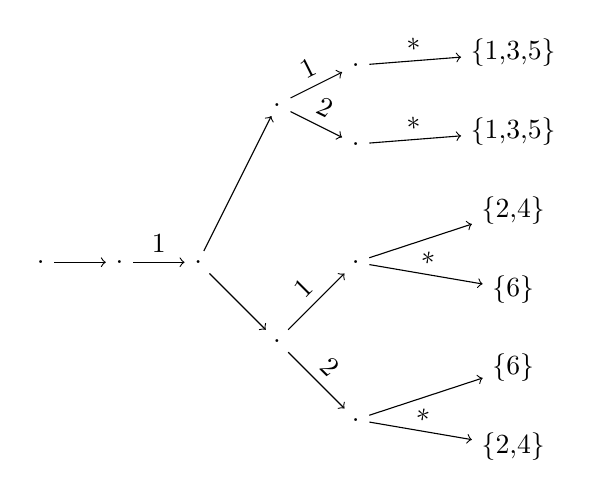
\begin{tikzpicture}[->,sloped,above]

	\node (root) at (0,2.5) {.};

	\node (h) at (1,2.5) {.};

	\node (h1) at (2,2.5) {.};

	\node (h1f) at (3,4.5) {.};
	\node (h1g) at (3,1.5) {.};

	\node (h1f1) at (4,5) {.};
	\node (h1f2) at (4,4) {.};
	\node (h1g1) at (4,2.5) {.};
	\node (h1g2) at (4,0.5) {.};

	\node (h1f1x) at (6,5) {\{1,3,5\}};
	\node (h1f2x) at (6,4) {\{1,3,5\}};
	\node (h1g1a) at (6,3) {\{2,4\}};
	\node (h1g1x) at (6,2) {\{6\}};
	\node (h1g2a) at (6,1) {\{6\}};
	\node (h1g2x) at (6,0) {\{2,4\}};

	\path (root) edge node {\( \mh \)} (h)
	(h) edge node {\( 1 \)} (h1)

	(h1)
	edge node {\( \mf \)} (h1f)
	edge node {\( \mg \)} (h1g)

	(h1f)
	edge node {\( 1 \)} (h1f1)
	edge node {\( 2 \)} (h1f2)

	(h1g)
	edge node {\( 1 \)} (h1g1)
	edge node {\( 2 \)} (h1g2)

	(h1f1)
	% edge node {\( \ma \)} (h1f1a)
	edge node {\( * \)} (h1f1x)

	(h1f2)
	%		edge node {\( \ma \)} (h1f2a)
	edge node {\( * \)} (h1f2x)


	(h1g1)
	edge node {\( \ma \)} (h1g1a)
	edge node {\( * \)} (h1g1x)

	(h1g2)
	edge node {\( \ma \)} (h1g2a)
	edge node {\( * \)} (h1g2x)
	;
	\end{tikzpicture}
\end{center}
\( \mh(\mg(y,x)) \mapsto \{ \mh.1.\mg.1.{*}, \mh.1.\mg.2.{*} \} \)
\end{example}

%+ PATH INDEXING/Retrieve
\begin{example}{Retrieve}
	\def\TRIEWIDTH{5cm}
	\def\TEXTWIDTH{\textwidth-\TRIEWIDTH-2em}

	\begin{minipage}{\TEXTWIDTH}
		\(
		\TI{t_1}\mh(\mf(x,y)),
		\TI{t_2}\mh(\mf({ x},{\ma})),
		\TI{t_3}\mh(\mf(\ma,\ma))
		 \)
		\begin{align*}
		\mh(\mf(z,\mb)) &\Rightarrow \{ \mh.1.\mf.1.{*}, \mh.1.\mf.2.\mb \}
		\\[0.7em]
		u : \mh(\mf({\colN z},{\colHi \mb}))
		& \mapsto
		{
			\{ t_1, {\colG t_2},
			{t_3} \}
		}
		{
			\cap \{t_1 \}
		}\\
%		{
			i : \mh(\mf(z, \mb)) &\mapsto \{ {\colG t_1,t_2,t_3 } \} \cap \{  \}
%		}
	\\
%		{
			g : \mh(\mf(z, \mb)) &\mapsto \{ t_1, {\colG t_2} \} \cap \{ t_1 \}
%		}
	\\
%		{
			v : \mh(\mf(z, \mb)) &\mapsto \{ {\colG t_1,t_2 }\} \cap \{  \}
%		}
	\\[0.7em]
%		{
			\colG v: \mh(\mf(z, z)) &\mapsto \{ {\colLo t_1},{\colG t_2} \} \cap \{ {\colLo t_1} \}
%		}
	\end{align*}
	\end{minipage}
	%
	\begin{minipage}{{\TRIEWIDTH}}
		\begin{tikzpicture}[->,dotted]
%		\ORIGIN

\def\pyL{-0.2}
\def\pxL{0.05}

\PAUSE

\node (root) at (2.5,5) {.};
\node (h) at (2.5,4) {.};
\path (root) edge node {$\mh$} (h);

\PAUSE
\node (h1) at (2.5,3) {.};
\path (h) edge node {$1$} (h1);

\PAUSE
\node (h1f) at (1.5,2) {.};
\path (h1) edge node {$\mf$} (h1f);

\PAUSE
\node (h1f1) at (0.5,1) {.};
\path (h1f) edge node {$1$} (h1f1);

\PAUSE
\node (h1f1x) at (0,0) {.};
\path (h1f1) edge node {$*$} (h1f1x);
\node (12) at (\pxL,\pyL) {\scriptsize$t_1,t_2$};

\PAUSE
\node (h1f1a) at (1,0) {.};
\path (h1f1) edge node {$\ma$} (h1f1a);
\node (3) at (\pxL+1,\pyL) {\scriptsize$t_3$};

\PAUSE
\node (h1f2) at (2.5,1) {.};
\path (h1f) edge node {$2$} (h1f2);

\PAUSE
\node (h1f2x) at (2,0) {.};
\path (h1f2) edge node {$*$} (h1f2x);
\node (1) at (\pxL+2,\pyL) {\scriptsize$t_1$};

\PAUSE
\node (h1f2a) at (3,0) {.};
\path (h1f2) edge node {$\ma$} (h1f2a);
\node (23) at (\pxL+3,\pyL) {\scriptsize$t_2,t_3$};


\node (lu) at (0,-0.5) {} ;
		\ORIGIN

\def\pyL{-0.2}
\def\pxL{0.05}

\node (root) at (2.5,5) {.};
\node (h) at (2.5,4) {.};
\path (root) edge node {$\mh$} (h);

\node (h1) at (2.5,3) {.};
\path (h) edge node {$1$} (h1);

\node (h1f) at (1.5,2) {.};
\path (h1) edge node {$\mf$} (h1f);

\node (h1f1) at (0.5,1) {.};
\path (h1f) edge node {$1$} (h1f1);

\node (h1f1x) at (0,0) {.};
\path (h1f1) edge node {$*$} (h1f1x);
\node (12) at (\pxL,\pyL) {\scriptsize$t_1,t_2$};

\node (h1f1a) at (1,0) {.};
\path (h1f1) edge node {$\ma$} (h1f1a);
\node (3) at (\pxL+1,\pyL) {\scriptsize$t_3$};

\node (h1f2) at (2.5,1) {.};
\path (h1f) edge node {$2$} (h1f2);

\node (h1f2x) at (2,0) {.};
\path (h1f2) edge node {$*$} (h1f2x);
\node (1) at (\pxL+2,\pyL) {\scriptsize$t_1$};

\node (h1f2a) at (3,0) {.};
\path (h1f2) edge node {$\ma$} (h1f2a);
\node (23) at (\pxL+3,\pyL) {\scriptsize$t_2,t_3$};

\node (lu) at (0,-0.5) {} ;

		\path[bend right, dashed, colN](root) edge (h);
		\node at (1.3,5) {\scriptsize\( (\mh,1.\mf.1.{*}) \)};
		\path[bend right, dashed, colN]	(h) edge (h1);
		\node at (1.0,4) {\scriptsize\( (1,\mf.1.{*}) \)};
		\path[bend right, dashed, colN]	(h1) edge (h1f);
		\node at (0.7,3) {\scriptsize\( (\mf,1.{*}) \)};
		\path[bend right, dashed, colN]	(h1f) edge (h1f1);
		\node at (0.4,2) {\scriptsize\( (1,{*}) \)};
		\path[bend right, dashed, colN]	(h1f1) edge (h1f1x)	;
		\node at (0.1,1) {\scriptsize\( ({*},\epsilon) \)};
		\path[bend right, dashed, colN]	(h1f1) edge (h1f1a);

		\path[bend left, dashed, colHi]	(root) edge (h)	;
		\node at (3.5,5) {\scriptsize\( (\mh,1.\mf.2.\mb) \)};
		\path[bend left, dashed, colHi]	(h) edge (h1)	;
		\node at (3.4,4) {\scriptsize\( (1,\mf.2.\mb) \)};
		\path[bend left, dashed, colHi]	(h1) edge (h1f)	;
		\node at (3.3,3) {\scriptsize\( (\mf,2.\mb) \)};
		\path[bend left, dashed, colHi]	(h1f) edge (h1f2)	;
		\node at (3.2,2) {\scriptsize\( (2,\mb) \)};
		\path[bend left, dashed, colHi]	(h1f2) edge (h1f2x)	;
		\node at (3.1,1) {\scriptsize\( (\mb,\epsilon) \)};
		\end{tikzpicture}
	\end{minipage}
\end{example}

%+ PATH INDEXING/Subterms
\begin{example}{Demodulation (Subterms)}

	\(
	\colG
	\TI{t_1}\mh(\mf(x,y)),
	\TI{t_2}\mh(\mf({ x},{\ma})),
	\TI{t_3}\mh(\mf(\ma,\ma)),
	\ldots,
%	\color{black}\mf(x,\ma) \foEQ x
	\color{black}\mf(x,\ma) \mEQ x
	 \)


	 \def\TRIEWIDTH{\textwidth/2-1em}% chktex 8
	 \def\TEXTWIDTH{\textwidth-\TRIEWIDTH-2em}
	\begin{minipage}{\TEXTWIDTH}
		\begin{tikzpicture}[->,dotted]
%		\ORIGIN

\def\pyL{-0.2}
\def\pxL{0.05}

\PAUSE

\node (root) at (2.5,5) {.};
\node (h) at (2.5,4) {.};
\path (root) edge node {$\mh$} (h);

\PAUSE
\node (h1) at (2.5,3) {.};
\path (h) edge node {$1$} (h1);

\PAUSE
\node (h1f) at (1.5,2) {.};
\path (h1) edge node {$\mf$} (h1f);

\PAUSE
\node (h1f1) at (0.5,1) {.};
\path (h1f) edge node {$1$} (h1f1);

\PAUSE
\node (h1f1x) at (0,0) {.};
\path (h1f1) edge node {$*$} (h1f1x);
\node (12) at (\pxL,\pyL) {\scriptsize$t_1,t_2$};

\PAUSE
\node (h1f1a) at (1,0) {.};
\path (h1f1) edge node {$\ma$} (h1f1a);
\node (3) at (\pxL+1,\pyL) {\scriptsize$t_3$};

\PAUSE
\node (h1f2) at (2.5,1) {.};
\path (h1f) edge node {$2$} (h1f2);

\PAUSE
\node (h1f2x) at (2,0) {.};
\path (h1f2) edge node {$*$} (h1f2x);
\node (1) at (\pxL+2,\pyL) {\scriptsize$t_1$};

\PAUSE
\node (h1f2a) at (3,0) {.};
\path (h1f2) edge node {$\ma$} (h1f2a);
\node (23) at (\pxL+3,\pyL) {\scriptsize$t_2,t_3$};


\node (lu) at (0,-0.5) {} ;
		\ORIGIN

\def\pyL{-0.2}
\def\pxL{0.05}

\node (root) at (2.5,5) {.};
\node (h) at (2.5,4) {.};
\path (root) edge node {$\mh$} (h);

\node (h1) at (2.5,3) {.};
\path (h) edge node {$1$} (h1);

\node (h1f) at (1.5,2) {.};
\path (h1) edge node {$\mf$} (h1f);

\node (h1f1) at (0.5,1) {.};
\path (h1f) edge node {$1$} (h1f1);

\node (h1f1x) at (0,0) {.};
\path (h1f1) edge node {$*$} (h1f1x);
\node (12) at (\pxL,\pyL) {\scriptsize$t_1,t_2$};

\node (h1f1a) at (1,0) {.};
\path (h1f1) edge node {$\ma$} (h1f1a);
\node (3) at (\pxL+1,\pyL) {\scriptsize$t_3$};

\node (h1f2) at (2.5,1) {.};
\path (h1f) edge node {$2$} (h1f2);

\node (h1f2x) at (2,0) {.};
\path (h1f2) edge node {$*$} (h1f2x);
\node (1) at (\pxL+2,\pyL) {\scriptsize$t_1$};

\node (h1f2a) at (3,0) {.};
\path (h1f2) edge node {$\ma$} (h1f2a);
\node (23) at (\pxL+3,\pyL) {\scriptsize$t_2,t_3$};

\node (lu) at (0,-0.5) {} ;

		\node (f) at (1.5,4) {.};
		\path[colN] (root) edge node {f} (f);

		\node (f1) at (0.5,4) {.};
		\path[colN] (f) edge node {1} (f1);

		\node (f1x) at (-0.5,4) {};
		\path[colN] (f1)	edge node {*} (f1x);

		\node[colN] (t1) at (-0.5,4.2) {\scriptsize\( t_1^1 \)};
		\node[colN] (t1) at (-0.5,3.8) {\scriptsize\(  t_2^1 \)};

		\node (f1a) at (-0.5,3) {};
		\path[colN] (f1) edge node {a} (f1a);

		\node[colN] (t3) at (-0.5,2.9) {\scriptsize\( t_3^1 \)};

		\node (f2) at (0.5,3) {.};
		\path[colN] (f) edge node {2}  (f2);

		\node (f2x) at (-0.5,2) {};
		\path[colN] (f2) edge node {*} (f2x);

		\node[colN] (t1) at (-0.5,1.9) {\scriptsize\( t_1^1 \)};

		\node (f2a) at (0.5,2) {};
		\path[colN] (f2) edge node {a} (f2a);

		\node[colN] (t2t3) at (0.5,1.9) {\scriptsize\( t_2^1,t_3^1 \)};

		\node (a) at (3.5,4) {};
		\path[colN] (root)  edge node {\( \ma \)} (a);
		\node[colN] (t2t3t3) at (3.5,3.9) {\scriptsize\( t_2^{12},t_3^{11,12} \)};

		\end{tikzpicture}
	\end{minipage}
	\hfill
	\begin{minipage}{{\TRIEWIDTH}}
		\def\pyL{-0.2}
		\def\pxL{0.05}
		\begin{tikzpicture}[->,dotted]
%		\ORIGIN

\def\pyL{-0.2}
\def\pxL{0.05}

\PAUSE

\node (root) at (2.5,5) {.};
\node (h) at (2.5,4) {.};
\path (root) edge node {$\mh$} (h);

\PAUSE
\node (h1) at (2.5,3) {.};
\path (h) edge node {$1$} (h1);

\PAUSE
\node (h1f) at (1.5,2) {.};
\path (h1) edge node {$\mf$} (h1f);

\PAUSE
\node (h1f1) at (0.5,1) {.};
\path (h1f) edge node {$1$} (h1f1);

\PAUSE
\node (h1f1x) at (0,0) {.};
\path (h1f1) edge node {$*$} (h1f1x);
\node (12) at (\pxL,\pyL) {\scriptsize$t_1,t_2$};

\PAUSE
\node (h1f1a) at (1,0) {.};
\path (h1f1) edge node {$\ma$} (h1f1a);
\node (3) at (\pxL+1,\pyL) {\scriptsize$t_3$};

\PAUSE
\node (h1f2) at (2.5,1) {.};
\path (h1f) edge node {$2$} (h1f2);

\PAUSE
\node (h1f2x) at (2,0) {.};
\path (h1f2) edge node {$*$} (h1f2x);
\node (1) at (\pxL+2,\pyL) {\scriptsize$t_1$};

\PAUSE
\node (h1f2a) at (3,0) {.};
\path (h1f2) edge node {$\ma$} (h1f2a);
\node (23) at (\pxL+3,\pyL) {\scriptsize$t_2,t_3$};


\node (lu) at (0,-0.5) {} ;
		\ORIGIN

\def\pyL{-0.2}
\def\pxL{0.05}

\node (root) at (2.5,5) {.};
\node (h) at (2.5,4) {.};
\path (root) edge node {$\mh$} (h);

\node (h1) at (2.5,3) {.};
\path (h) edge node {$1$} (h1);

\node (h1f) at (1.5,2) {.};
\path (h1) edge node {$\mf$} (h1f);

\node (h1f1) at (0.5,1) {.};
\path (h1f) edge node {$1$} (h1f1);

\node (h1f1x) at (0,0) {.};
\path (h1f1) edge node {$*$} (h1f1x);
\node (12) at (\pxL,\pyL) {\scriptsize$t_1,t_2$};

\node (h1f1a) at (1,0) {.};
\path (h1f1) edge node {$\ma$} (h1f1a);
\node (3) at (\pxL+1,\pyL) {\scriptsize$t_3$};

\node (h1f2) at (2.5,1) {.};
\path (h1f) edge node {$2$} (h1f2);

\node (h1f2x) at (2,0) {.};
\path (h1f2) edge node {$*$} (h1f2x);
\node (1) at (\pxL+2,\pyL) {\scriptsize$t_1$};

\node (h1f2a) at (3,0) {.};
\path (h1f2) edge node {$\ma$} (h1f2a);
\node (23) at (\pxL+3,\pyL) {\scriptsize$t_2,t_3$};

\node (lu) at (0,-0.5) {} ;

		\node[colN] (n-hsubs) at (5,4) {\( \mh \)};
		\path[dashdotted, above, pos=0.3,sloped,bend right=5,colN]  (n-hsubs) edge node {\scriptsize\( \ANGLES{\epsilon,\mh} \)} (h);

		\node[colN] (n-fsubs) at (5,3) {\( \mf \)};
		\path[dashdotted, above, pos=0.3,sloped, bend right=10,colN]  (n-fsubs) edge node {\scriptsize\( \ANGLES{1,\mf} \)} (h1f);

		\node[colN] (n-asubs) at (5,2) {\( \ma \)};
		\path[dashdotted, above, bend right, pos=0.3,sloped,colN]  (n-asubs) edge node {\scriptsize\( \ANGLES{11,\ma} \)} (h1f1a);
		\path[dashdotted, bend right, below, pos=0.3,sloped,colN]  (n-asubs) edge node {\scriptsize\( \ANGLES{12,\ma} \)} (h1f2a);

		\end{tikzpicture}
	\end{minipage}


\end{example}

%+ PATH INDEXING/SubtermTrees
\begin{example}{Subterm trees}
\begin{gather*}
\{
\TI{1}\mh(\mf(x,x)),
\TI{2}\mh(\mg(\ma,x)),
\TI{3}\mh(\mf(y,z))
\TI{4}\mh(\mg(\ma,y)),
\TI{5}\mh(\mf(y,x)),
\TI{6}\mh(\mg(y,a))
\}
\end{gather*}
%
\begin{center}
	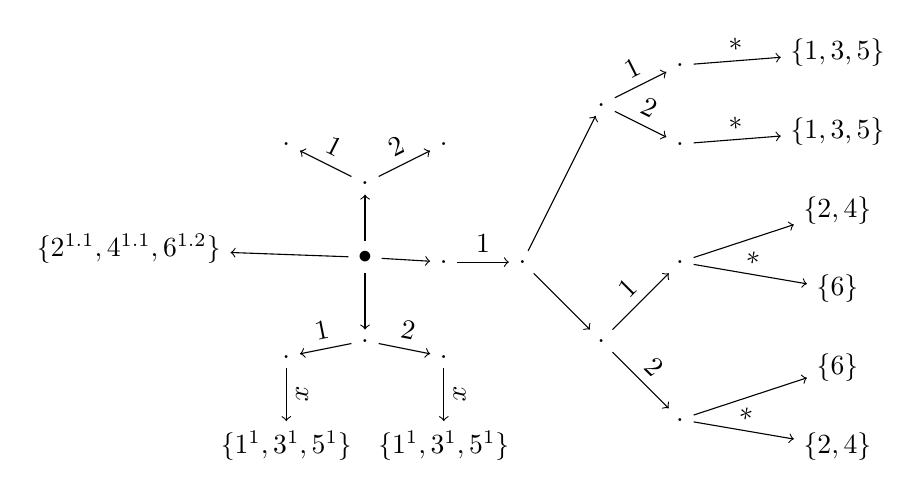
\begin{tikzpicture}[->,sloped,above]
	\node (root) at (0,2.5) {\( \bullet \)};
	%% right
	\node (h) at (1,2.5) {.};
	%
	\node (h1) at (2,2.5) {.};
	%
	\node (h1f) at (3,4.5) {.};
	\node (h1g) at (3,1.5) {.};
	%
	\node (h1f1) at (4,5) {.};
	\node (h1f2) at (4,4) {.};
	\node (h1g1) at (4,2.5) {.};
	\node (h1g2) at (4,0.5) {.};
	%
	\node (h1f1x) at (6,5) {\( \{1,3,5\} \)};
	\node (h1f2x) at (6,4) {\( \{1,3,5\} \)};
	\node (h1g1a) at (6,3) {\( \{2,4\} \)};
	\node (h1g1x) at (6,2) {\( \{6\} \)};
	\node (h1g2a) at (6,1) {\( \{6\} \)};
	\node (h1g2x) at (6,0) {\( \{2,4\} \)};
	%% down
	\node (f) at (0,1.5) {.};
	\node (f1) at (-1,1.3) {.};
	\node (f1x) at (-1,0) {\( \{1^{1},3^{1},5^{1}\} \)};
	\node (f2) at (1,1.3) {.};
	\node (f2x) at (1,0) {\( \{1^{1},3^{1},5^{1}\} \)};
	%% up
	\node (g) at (0,3.5) {.};
	\node (g1) at (-1,4) {.};
	\node (g2) at (1,4) {.};
	%% left
	\node (a) at (-3,2.5) {\( \{2^{1.1}, 4^{1.1}, 6^{1.2}\} \)};

	\path
	(root)
	edge node {\( \mh \)} (h)
	edge node {\( \mf \)} (f)
	edge node {\( \mg \)} (g)
	edge node {\( \ma \)} (a)

	(h) edge node {\( 1 \)} (h1)


	(h1)
	edge node {\( \mf \)} (h1f)
	edge node {\( \mg \)} (h1g)

	(h1f)
	edge node {\( 1 \)} (h1f1)
	edge node {\( 2 \)} (h1f2)

	(h1g)
	edge node {\( 1 \)} (h1g1)
	edge node {\( 2 \)} (h1g2)

	(h1f1)
	edge node {\( * \)} (h1f1x)

	(h1f2)
	edge node {\( * \)} (h1f2x)


	(h1g1)
	edge node {\( \ma \)} (h1g1a)
	edge node {\( * \)} (h1g1x)

	(h1g2)
	edge node {\( \ma \)} (h1g2a)
	edge node {\( * \)} (h1g2x)

	%
	(g) 	edge node {\( 1 \)} (g1)
	edge node {\( 2 \)} (g2)

	(f)	edge node {\( 1 \)} (f1)
	edge node {\( 2 \)} (f2)

	(f1)	edge node {\( x \)} (f1x)
	(f2)	edge node {\( x \)} (f2x)
	;


	\path (root)



	;

	\end{tikzpicture}
\end{center}
\end{example}





\subsection{Substitution Tree}
%% SUBSTITUTION TREES

%+ SUBSTITUTION TREES/Build+Index
\begin{example}{Substitution tree build}

	\(
	\TI{t_1}\mh(\mf(x,y)),
	\TI{t_2}\mh(\mf(x,\mh(\ma))),
	\TI{t_3}\mh(\mf(\mh(\ma),\ma)),
	\TI{t_4}\mh(\mf(\ma,\ma))
	 \)

	\begin{tikzpicture}[->]
%	\ORIGIN

\def\pyL{-0.2}
\def\pxL{0.05}

\PAUSE

\node (root) at (2.5,5) {.};
\node (h) at (2.5,4) {.};
\path (root) edge node {$\mh$} (h);

\PAUSE
\node (h1) at (2.5,3) {.};
\path (h) edge node {$1$} (h1);

\PAUSE
\node (h1f) at (1.5,2) {.};
\path (h1) edge node {$\mf$} (h1f);

\PAUSE
\node (h1f1) at (0.5,1) {.};
\path (h1f) edge node {$1$} (h1f1);

\PAUSE
\node (h1f1x) at (0,0) {.};
\path (h1f1) edge node {$*$} (h1f1x);
\node (12) at (\pxL,\pyL) {\scriptsize$t_1,t_2$};

\PAUSE
\node (h1f1a) at (1,0) {.};
\path (h1f1) edge node {$\ma$} (h1f1a);
\node (3) at (\pxL+1,\pyL) {\scriptsize$t_3$};

\PAUSE
\node (h1f2) at (2.5,1) {.};
\path (h1f) edge node {$2$} (h1f2);

\PAUSE
\node (h1f2x) at (2,0) {.};
\path (h1f2) edge node {$*$} (h1f2x);
\node (1) at (\pxL+2,\pyL) {\scriptsize$t_1$};

\PAUSE
\node (h1f2a) at (3,0) {.};
\path (h1f2) edge node {$\ma$} (h1f2a);
\node (23) at (\pxL+3,\pyL) {\scriptsize$t_2,t_3$};


\node (lu) at (0,-0.5) {} ;
	\ORIGIN


\node (root) at (0,0) {.};
\node (h) at (0,-1) {\( *_0 \mapsto \mh(*_1) \)};
\path (root) edge (h);

\node (f) at (0,-2) {\( *_1 \mapsto \mf(*_2,*_3) \)};
\path (h) edge (f);

\node (x2x) at (-2,-3) {\( *_2 \mapsto x \)} ;
\path (f) edge (x2x);

\node (x3y) at (-3,-4) {\( *_3 \mapsto y \)};
\path (x2x) edge (x3y);
\node (t1) at (-3,-4.4) {\( t_1 \)};

\node (x3ha) at (-1,-4) {\( *_3 \mapsto \mh(\ma) \)};
\path (x2x) edge (x3ha);
\node (t2) at (-1,-4.4) {\( t_2 \)};

\node (x3a)at (2,-3) {\( *_3\mapsto\ma \)};
\path (f) edge (x3a);

\node (x2ha) at (1,-4) {\( *_2\mapsto\mh(\ma) \)};
\path (x3a) edge (x2ha);
\node (t3) at (1,-4.4) {\( t_3 \)};

\node (x2a) at (3,-4) {\( *_2\mapsto\ma \)};
\path (x3a) edge (x2a);
\node (t4) at (3,-4.4) {\( t_4 \)};

	\end{tikzpicture}
\end{example}

%+ SUBSTITUTION TREES/Retrieve+Index
\begin{example}{Substitution tree retrieve}

	\(
	\TI{t_1}\mh(\mf(x,y)),
	\TI{t_2}\mh(\mf(x,\mh(\ma))),
	\TI{t_3}\mh(\mf(\mh(\ma),\ma)),
	\TI{t_4}\mh(\mf(\ma,\ma))
	 \)

	\begin{tikzpicture}[->]
%	\ORIGIN

\def\pyL{-0.2}
\def\pxL{0.05}

\PAUSE

\node (root) at (2.5,5) {.};
\node (h) at (2.5,4) {.};
\path (root) edge node {$\mh$} (h);

\PAUSE
\node (h1) at (2.5,3) {.};
\path (h) edge node {$1$} (h1);

\PAUSE
\node (h1f) at (1.5,2) {.};
\path (h1) edge node {$\mf$} (h1f);

\PAUSE
\node (h1f1) at (0.5,1) {.};
\path (h1f) edge node {$1$} (h1f1);

\PAUSE
\node (h1f1x) at (0,0) {.};
\path (h1f1) edge node {$*$} (h1f1x);
\node (12) at (\pxL,\pyL) {\scriptsize$t_1,t_2$};

\PAUSE
\node (h1f1a) at (1,0) {.};
\path (h1f1) edge node {$\ma$} (h1f1a);
\node (3) at (\pxL+1,\pyL) {\scriptsize$t_3$};

\PAUSE
\node (h1f2) at (2.5,1) {.};
\path (h1f) edge node {$2$} (h1f2);

\PAUSE
\node (h1f2x) at (2,0) {.};
\path (h1f2) edge node {$*$} (h1f2x);
\node (1) at (\pxL+2,\pyL) {\scriptsize$t_1$};

\PAUSE
\node (h1f2a) at (3,0) {.};
\path (h1f2) edge node {$\ma$} (h1f2a);
\node (23) at (\pxL+3,\pyL) {\scriptsize$t_2,t_3$};


\node (lu) at (0,-0.5) {} ;
	\ORIGIN


\node (root) at (0,0) {.};
\node (h) at (0,-1) {\( *_0 \mapsto \mh(*_1) \)};
\path (root) edge (h);

\node (f) at (0,-2) {\( *_1 \mapsto \mf(*_2,*_3) \)};
\path (h) edge (f);

\node (x2x) at (-2,-3) {\( *_2 \mapsto x \)} ;
\path (f) edge (x2x);

\node (x3y) at (-3,-4) {\( *_3 \mapsto y \)};
\path (x2x) edge (x3y);
\node (t1) at (-3,-4.4) {\( t_1 \)};

\node (x3ha) at (-1,-4) {\( *_3 \mapsto \mh(\ma) \)};
\path (x2x) edge (x3ha);
\node (t2) at (-1,-4.4) {\( t_2 \)};

\node (x3a)at (2,-3) {\( *_3\mapsto\ma \)};
\path (f) edge (x3a);

\node (x2ha) at (1,-4) {\( *_2\mapsto\mh(\ma) \)};
\path (x3a) edge (x2ha);
\node (t3) at (1,-4.4) {\( t_3 \)};

\node (x2a) at (3,-4) {\( *_2\mapsto\ma \)};
\path (x3a) edge (x2a);
\node (t4) at (3,-4.4) {\( t_4 \)};
	\end{tikzpicture}
\end{example}

%% DISCRIMINATION TREE
\subsection{Discrimination Tree}

%\ORIGIN

\node (root) at (1,0) {.};
\node (h) at (0,-1) {.};
\path (root) edge node {\( \mh \)} (h);
\node (hf) at (-1,-2) {.};
\path (h) edge node {\( \mf \)} (hf);
\node (hfx) at (-2,-3) {.};
\path (hf) edge node {\( * \)} (hfx);
\node (n-hfxx) at (-3,-4) {.};
\path (hfx) edge node {\( * \)} (n-hfxx);
\node (1) at (-3,-4.2) {\scriptsize \( t_1 \)};

\node (n-hfxh) at (-2,-4) {.};
\path (hfx) edge node {\( \mh \)} (n-hfxh);
\node (n-hfxha) at (-2,-5) {.};
\path (n-hfxh) edge node {\( \ma \)} (n-hfxha);
\node (2) at (-2,-5.2) {\scriptsize \( t_2 \)};

\node (hfh) at (-1,-3) {.};
\path (hf) edge node {\( \mh \)} (hfh);
\node (n-hfha) at (-1,-4) {.};
\path (hfh) edge node {\( \ma \)} (n-hfha);
\path[dashdotted,bend left=45,gray] (hf) edge (n-hfha);
\node (n-hfhaa) at (-1,-5) {.};
\path (n-hfha) edge node {\( \ma \)} (n-hfhaa);
\node (3) at (-1,-5.2) {\scriptsize \( t_3 \)};
%\(
\TI{t_1}\mh(\mf(x,y)),
\TI{t_2}\mh(\mf(x,\mh(\ma))),
\TI{t_3}\mh(\mf(\mh(\ma),\ma))
\)
%% DISCRIMINATION TREE/Build+Terms+Index
\begin{example}{Build}

	\def\TRIEWIDTH{4.4cm}
	\def\TEXTWIDTH{\textwidth-\TRIEWIDTH-2em}
	\begin{minipage}{\TEXTWIDTH}
%		$
\TI{\ell_1}\mP(\mf(x,y)), 
\TI{\ell_2}\mP(\mf(x,\mh(\ma))),
\TI{\ell_3}\mP(\mf(\mh(\ma),\ma))
$
		\(
\TI{t_1}\mh(\mf(x,y)),
\TI{t_2}\mh(\mf(x,\mh(\ma))),
\TI{t_3}\mh(\mf(\mh(\ma),\ma))
\)
		\begin{align*}
		t_1 &\Rightarrow \mh.\mf.{*}.{*}\\
		t_2 &\Rightarrow \mh.\mf.{*}.\mh.\ma \\
		t_3 &\Rightarrow \mh.\mf.\mh.\ma.\ma
		\end{align*}
	\end{minipage}
	\begin{minipage}{\TRIEWIDTH}
		\def\pyL{-0.3}
		\def\pxL{-0.0}
		\begin{tikzpicture}[->,dotted]
%		\ORIGIN

\def\pyL{-0.2}
\def\pxL{0.05}

\PAUSE

\node (root) at (2.5,5) {.};
\node (h) at (2.5,4) {.};
\path (root) edge node {$\mh$} (h);

\PAUSE
\node (h1) at (2.5,3) {.};
\path (h) edge node {$1$} (h1);

\PAUSE
\node (h1f) at (1.5,2) {.};
\path (h1) edge node {$\mf$} (h1f);

\PAUSE
\node (h1f1) at (0.5,1) {.};
\path (h1f) edge node {$1$} (h1f1);

\PAUSE
\node (h1f1x) at (0,0) {.};
\path (h1f1) edge node {$*$} (h1f1x);
\node (12) at (\pxL,\pyL) {\scriptsize$t_1,t_2$};

\PAUSE
\node (h1f1a) at (1,0) {.};
\path (h1f1) edge node {$\ma$} (h1f1a);
\node (3) at (\pxL+1,\pyL) {\scriptsize$t_3$};

\PAUSE
\node (h1f2) at (2.5,1) {.};
\path (h1f) edge node {$2$} (h1f2);

\PAUSE
\node (h1f2x) at (2,0) {.};
\path (h1f2) edge node {$*$} (h1f2x);
\node (1) at (\pxL+2,\pyL) {\scriptsize$t_1$};

\PAUSE
\node (h1f2a) at (3,0) {.};
\path (h1f2) edge node {$\ma$} (h1f2a);
\node (23) at (\pxL+3,\pyL) {\scriptsize$t_2,t_3$};


\node (lu) at (0,-0.5) {} ;
		\ORIGIN

\node (root) at (1,0) {.};
\node (h) at (0,-1) {.};
\path (root) edge node {\( \mh \)} (h);
\node (hf) at (-1,-2) {.};
\path (h) edge node {\( \mf \)} (hf);
\node (hfx) at (-2,-3) {.};
\path (hf) edge node {\( * \)} (hfx);
\node (n-hfxx) at (-3,-4) {.};
\path (hfx) edge node {\( * \)} (n-hfxx);
\node (1) at (-3,-4.2) {\scriptsize \( t_1 \)};

\node (n-hfxh) at (-2,-4) {.};
\path (hfx) edge node {\( \mh \)} (n-hfxh);
\node (n-hfxha) at (-2,-5) {.};
\path (n-hfxh) edge node {\( \ma \)} (n-hfxha);
\node (2) at (-2,-5.2) {\scriptsize \( t_2 \)};

\node (hfh) at (-1,-3) {.};
\path (hf) edge node {\( \mh \)} (hfh);
\node (n-hfha) at (-1,-4) {.};
\path (hfh) edge node {\( \ma \)} (n-hfha);
\path[dashdotted,bend left=45,gray] (hf) edge (n-hfha);
\node (n-hfhaa) at (-1,-5) {.};
\path (n-hfha) edge node {\( \ma \)} (n-hfhaa);
\node (3) at (-1,-5.2) {\scriptsize \( t_3 \)};
		\node (lu) at (-3,-5.5) {} ;
		\end{tikzpicture}
	\end{minipage}
	%
\end{example}



%% DISCRIMINATION TREE/Index
%% DISCRIMINATION TREE/IndexEdges

%+ DISCRIMINATION TREE/Retrieve+Terms+Index
\begin{example}{Retrieve}

	\def\TRIEWIDTH{4.4cm}
	\def\TEXTWIDTH{\textwidth-\TRIEWIDTH-2em}
	\begin{minipage}{\TEXTWIDTH}
%		$
\TI{\ell_1}\mP(\mf(x,y)), 
\TI{\ell_2}\mP(\mf(x,\mh(\ma))),
\TI{\ell_3}\mP(\mf(\mh(\ma),\ma))
$
		\(
\TI{t_1}\mh(\mf(x,y)),
\TI{t_2}\mh(\mf(x,\mh(\ma))),
\TI{t_3}\mh(\mf(\mh(\ma),\ma))
\)
		\begin{align*}
		\mh(\mf(x',\ma))&\Rightarrow \mh.\mf.{*}.\ma
		\\[0.7em]
		u: \mh(\mf(x',\ma))&\mapsto \{
		{t_1,}
		{t_3}
		\}
		\\
					i:\mh(\mf(x',\ma))&\mapsto \{t_3\}  \\
					g:\mh(\mf(x',\ma))&\mapsto \{t_1\} \\
					v:\mh(\mf(x',\ma))&\mapsto \{  \} \\
		\end{align*}
	\end{minipage}
%
	\begin{minipage}{\TRIEWIDTH}
		\begin{tikzpicture}[->,dotted]
%		\ORIGIN

\def\pyL{-0.2}
\def\pxL{0.05}

\PAUSE

\node (root) at (2.5,5) {.};
\node (h) at (2.5,4) {.};
\path (root) edge node {$\mh$} (h);

\PAUSE
\node (h1) at (2.5,3) {.};
\path (h) edge node {$1$} (h1);

\PAUSE
\node (h1f) at (1.5,2) {.};
\path (h1) edge node {$\mf$} (h1f);

\PAUSE
\node (h1f1) at (0.5,1) {.};
\path (h1f) edge node {$1$} (h1f1);

\PAUSE
\node (h1f1x) at (0,0) {.};
\path (h1f1) edge node {$*$} (h1f1x);
\node (12) at (\pxL,\pyL) {\scriptsize$t_1,t_2$};

\PAUSE
\node (h1f1a) at (1,0) {.};
\path (h1f1) edge node {$\ma$} (h1f1a);
\node (3) at (\pxL+1,\pyL) {\scriptsize$t_3$};

\PAUSE
\node (h1f2) at (2.5,1) {.};
\path (h1f) edge node {$2$} (h1f2);

\PAUSE
\node (h1f2x) at (2,0) {.};
\path (h1f2) edge node {$*$} (h1f2x);
\node (1) at (\pxL+2,\pyL) {\scriptsize$t_1$};

\PAUSE
\node (h1f2a) at (3,0) {.};
\path (h1f2) edge node {$\ma$} (h1f2a);
\node (23) at (\pxL+3,\pyL) {\scriptsize$t_2,t_3$};


\node (lu) at (0,-0.5) {} ;
		\ORIGIN

\node (root) at (1,0) {.};
\node (h) at (0,-1) {.};
\path (root) edge node {\( \mh \)} (h);
\node (hf) at (-1,-2) {.};
\path (h) edge node {\( \mf \)} (hf);
\node (hfx) at (-2,-3) {.};
\path (hf) edge node {\( * \)} (hfx);
\node (n-hfxx) at (-3,-4) {.};
\path (hfx) edge node {\( * \)} (n-hfxx);
\node (1) at (-3,-4.2) {\scriptsize \( t_1 \)};

\node (n-hfxh) at (-2,-4) {.};
\path (hfx) edge node {\( \mh \)} (n-hfxh);
\node (n-hfxha) at (-2,-5) {.};
\path (n-hfxh) edge node {\( \ma \)} (n-hfxha);
\node (2) at (-2,-5.2) {\scriptsize \( t_2 \)};

\node (hfh) at (-1,-3) {.};
\path (hf) edge node {\( \mh \)} (hfh);
\node (n-hfha) at (-1,-4) {.};
\path (hfh) edge node {\( \ma \)} (n-hfha);
\path[dashdotted,bend left=45,gray] (hf) edge (n-hfha);
\node (n-hfhaa) at (-1,-5) {.};
\path (n-hfha) edge node {\( \ma \)} (n-hfhaa);
\node (3) at (-1,-5.2) {\scriptsize \( t_3 \)};
		\path[bend right, dashed, colN] (root) edge  (h);
		\path[bend right, dashed, colN] (h) edge  (hf);
		\path[bend right, dashed, colN] (hf) edge (hfx);
		\path[bend right, dashed, colN] (hfx) edge  (n-hfxx);
		\path[bend right, dashed, colN] (hf) edge  (n-hfha);
		\path[bend right, dashed, colN] (n-hfha) edge (n-hfhaa);

		\node (lu) at (-3,-5.5) {} ;
		\end{tikzpicture}
	\end{minipage}
	%
\end{example}

%% DISCRIMINATION TREE/Subterms+Terms+Index
\begin{example}{Subterms}
	\def\TRIEWIDTH{\textwidth/2-1em}% chktex 8
%%	$
\TI{\ell_1}\mP(\mf(x,y)), 
\TI{\ell_2}\mP(\mf(x,\mh(\ma))),
\TI{\ell_3}\mP(\mf(\mh(\ma),\ma))
$
	\(
\TI{t_1}\mh(\mf(x,y)),
\TI{t_2}\mh(\mf(x,\mh(\ma))),
\TI{t_3}\mh(\mf(\mh(\ma),\ma))
\)
%	\vspace{1em}

	\begin{minipage}{\TRIEWIDTH}
		\begin{tikzpicture}[->, dotted]
%		\ORIGIN

\def\pyL{-0.2}
\def\pxL{0.05}

\PAUSE

\node (root) at (2.5,5) {.};
\node (h) at (2.5,4) {.};
\path (root) edge node {$\mh$} (h);

\PAUSE
\node (h1) at (2.5,3) {.};
\path (h) edge node {$1$} (h1);

\PAUSE
\node (h1f) at (1.5,2) {.};
\path (h1) edge node {$\mf$} (h1f);

\PAUSE
\node (h1f1) at (0.5,1) {.};
\path (h1f) edge node {$1$} (h1f1);

\PAUSE
\node (h1f1x) at (0,0) {.};
\path (h1f1) edge node {$*$} (h1f1x);
\node (12) at (\pxL,\pyL) {\scriptsize$t_1,t_2$};

\PAUSE
\node (h1f1a) at (1,0) {.};
\path (h1f1) edge node {$\ma$} (h1f1a);
\node (3) at (\pxL+1,\pyL) {\scriptsize$t_3$};

\PAUSE
\node (h1f2) at (2.5,1) {.};
\path (h1f) edge node {$2$} (h1f2);

\PAUSE
\node (h1f2x) at (2,0) {.};
\path (h1f2) edge node {$*$} (h1f2x);
\node (1) at (\pxL+2,\pyL) {\scriptsize$t_1$};

\PAUSE
\node (h1f2a) at (3,0) {.};
\path (h1f2) edge node {$\ma$} (h1f2a);
\node (23) at (\pxL+3,\pyL) {\scriptsize$t_2,t_3$};


\node (lu) at (0,-0.5) {} ;
		\ORIGIN

\node (root) at (1,0) {.};
\node (h) at (0,-1) {.};
\path (root) edge node {\( \mh \)} (h);
\node (hf) at (-1,-2) {.};
\path (h) edge node {\( \mf \)} (hf);
\node (hfx) at (-2,-3) {.};
\path (hf) edge node {\( * \)} (hfx);
\node (n-hfxx) at (-3,-4) {.};
\path (hfx) edge node {\( * \)} (n-hfxx);
\node (1) at (-3,-4.2) {\scriptsize \( t_1 \)};

\node (n-hfxh) at (-2,-4) {.};
\path (hfx) edge node {\( \mh \)} (n-hfxh);
\node (n-hfxha) at (-2,-5) {.};
\path (n-hfxh) edge node {\( \ma \)} (n-hfxha);
\node (2) at (-2,-5.2) {\scriptsize \( t_2 \)};

\node (hfh) at (-1,-3) {.};
\path (hf) edge node {\( \mh \)} (hfh);
\node (n-hfha) at (-1,-4) {.};
\path (hfh) edge node {\( \ma \)} (n-hfha);
\path[dashdotted,bend left=45,gray] (hf) edge (n-hfha);
\node (n-hfhaa) at (-1,-5) {.};
\path (n-hfha) edge node {\( \ma \)} (n-hfhaa);
\node (3) at (-1,-5.2) {\scriptsize \( t_3 \)};
		\node (ha) at (1,-2) {.} ;
		\path[dashdotted,colN] (h) edge node {\( \ma \)} (ha);
		\node (tha)  at (1,-2.2) {\scriptsize\( t_2^{{\colN 12}}, t_3^{{\colN 111}} \)} ;
		{(lu) at (-3.5,-5.5) {+}}

		\end{tikzpicture}
	\end{minipage}
%	\hfill{
		\begin{minipage}{\TRIEWIDTH}
			\begin{tikzpicture}[->,dotted]
%
%%			\ORIGIN

\def\pyL{-0.2}
\def\pxL{0.05}

\PAUSE

\node (root) at (2.5,5) {.};
\node (h) at (2.5,4) {.};
\path (root) edge node {$\mh$} (h);

\PAUSE
\node (h1) at (2.5,3) {.};
\path (h) edge node {$1$} (h1);

\PAUSE
\node (h1f) at (1.5,2) {.};
\path (h1) edge node {$\mf$} (h1f);

\PAUSE
\node (h1f1) at (0.5,1) {.};
\path (h1f) edge node {$1$} (h1f1);

\PAUSE
\node (h1f1x) at (0,0) {.};
\path (h1f1) edge node {$*$} (h1f1x);
\node (12) at (\pxL,\pyL) {\scriptsize$t_1,t_2$};

\PAUSE
\node (h1f1a) at (1,0) {.};
\path (h1f1) edge node {$\ma$} (h1f1a);
\node (3) at (\pxL+1,\pyL) {\scriptsize$t_3$};

\PAUSE
\node (h1f2) at (2.5,1) {.};
\path (h1f) edge node {$2$} (h1f2);

\PAUSE
\node (h1f2x) at (2,0) {.};
\path (h1f2) edge node {$*$} (h1f2x);
\node (1) at (\pxL+2,\pyL) {\scriptsize$t_1$};

\PAUSE
\node (h1f2a) at (3,0) {.};
\path (h1f2) edge node {$\ma$} (h1f2a);
\node (23) at (\pxL+3,\pyL) {\scriptsize$t_2,t_3$};


\node (lu) at (0,-0.5) {} ;
			\ORIGIN

\node (root) at (1,0) {.};
\node (h) at (0,-1) {.};
\path (root) edge node {\( \mh \)} (h);
\node (hf) at (-1,-2) {.};
\path (h) edge node {\( \mf \)} (hf);
\node (hfx) at (-2,-3) {.};
\path (hf) edge node {\( * \)} (hfx);
\node (n-hfxx) at (-3,-4) {.};
\path (hfx) edge node {\( * \)} (n-hfxx);
\node (1) at (-3,-4.2) {\scriptsize \( t_1 \)};

\node (n-hfxh) at (-2,-4) {.};
\path (hfx) edge node {\( \mh \)} (n-hfxh);
\node (n-hfxha) at (-2,-5) {.};
\path (n-hfxh) edge node {\( \ma \)} (n-hfxha);
\node (2) at (-2,-5.2) {\scriptsize \( t_2 \)};

\node (hfh) at (-1,-3) {.};
\path (hf) edge node {\( \mh \)} (hfh);
\node (n-hfha) at (-1,-4) {.};
\path (hfh) edge node {\( \ma \)} (n-hfha);
\path[dashdotted,bend left=45,gray] (hf) edge (n-hfha);
\node (n-hfhaa) at (-1,-5) {.};
\path (n-hfha) edge node {\( \ma \)} (n-hfhaa);
\node (3) at (-1,-5.2) {\scriptsize \( t_3 \)};
			\node (n-hsubs) at (1,-4.5) {};
			\path[dashdotted, colN, sloped,above] (n-hsubs)
			edge[pos=0.4] node[sloped]
			{\scriptsize\( \ANGLES{\epsilon,\mh} \)}  (h);
			\path[dashdotted, colN,sloped, above] (n-hsubs)
			edge[bend left=0,pos=0.4,sloped]
			node
			{\scriptsize\( \ANGLES{11,\mh} \)}
			(hfh);
%
			\path[dashdotted, colN] (n-hsubs)
			edge[bend left=0,pos=0.2,sloped]
			node[below] {\scriptsize \( \ANGLES{12,\mh} \)}
			(n-hfxh);
%
			\node (lu) at (-3.5,-5.5) {} ;
			\end{tikzpicture}
	\end{minipage}
%	%
\end{example}














\subsection{Clashing literals}

\subsection{Variants}

\subsection{Instances}

\subsection{Subsumption}



